
%\documentclass[mathserif]{beamer}
\documentclass[handout]{beamer}
%\usetheme{Goettingen}
%\usetheme{Warsaw}
\usetheme{Singapore}



%\usetheme{Frankfurt}
%\usetheme{Copenhagen}
%\usetheme{Szeged}
%\usetheme{Montpellier}
%\usetheme{CambridgeUS}
%\usecolortheme{}
%\setbeamercovered{transparent}
\usepackage[english, activeacute]{babel}
\usepackage[utf8]{inputenc}
\usepackage{amsmath, amssymb}
\usepackage{dsfont}
\usepackage{graphics}
\usepackage{cases}
\usepackage{graphicx}
\usepackage{pgf}
\usepackage{epsfig}
\usepackage{amssymb}
\usepackage{multirow}	
\usepackage{amstext}
\usepackage[ruled,vlined,lined]{algorithm2e}
\usepackage{amsmath}
\usepackage{epic}
\usepackage{epsfig}
\usepackage{fontenc}
\usepackage{framed,color}
\usepackage{palatino, url, multicol}
%\algsetup{indent=2em}
\newcommand{\factorial}{\ensuremath{\mbox{\sc Factorial}}}
\newcommand{\BIGOP}[1]{\mathop{\mathchoice%
{\raise-0.22em\hbox{\huge $#1$}}%
{\raise-0.05em\hbox{\Large $#1$}}{\hbox{\large $#1$}}{#1}}}
\newcommand{\bigtimes}{\BIGOP{\times}}
\vspace{-0.5cm}
\title{Natural Language Processing \\ Probabilistic Language Models}
\vspace{-0.5cm}
\author[Felipe Bravo Márquez]{\footnotesize
%\author{\footnotesize  
 \textcolor[rgb]{0.00,0.00,1.00}{Felipe Bravo-Marquez}} 
  
 

\date{\today}

\begin{document}
\begin{frame}
\titlepage


\end{frame}



\begin{frame}{Overview}
\begin{scriptsize}
\begin{itemize}
\item The language modeling problem
\item Trigram models
\item Evaluating language models: perplexity
\item  Estimation techniques:
\begin{enumerate}\scriptsize{
\item Linear interpolation
\item  Discounting methods}
\end{enumerate}
\item This slides are based on the course material by Michael Collins: \url{http://www.cs.columbia.edu/~mcollins/cs4705-spring2019/slides/lmslides.pdf} 

\end{itemize}
\end{scriptsize}
\end{frame}

\begin{frame}{The Language Modeling Problem}

\begin{scriptsize}
\begin{itemize}
\item We have some (finite) vocabulary, say $\mathcal{V}$ = $\{$the, a, man, telescope, Beckham, two, . . .$\}$
\item We have an (infinite) set of strings, $\mathcal{V}^*$.
\item For example: 
\begin{itemize}\scriptsize{
 \item the STOP 
\item a STOP 
\item the fan STOP
\item the fan saw Beckham STOP
\item the fan saw saw STOP
\item the fan saw Beckham play for Real Madrid STOP}
\end{itemize}
\item Where STOP is a special symbol indicating the end of a sentence.

\end{itemize}
\end{scriptsize}

\end{frame}


\begin{frame}{The Language Modeling Problem (Continued)}
\begin{scriptsize}
\begin{itemize}
\item We have a training sample of example sentences in English.
\item We need to "learn" a probability distribution $p$.
\item $p$ is a function that satisfies:
\begin{align*}
\sum_{x\in V^*} p(x) &= 1 \\
p(x) &\geq 0 \quad \text{for all } x \in V^*
\end{align*}


\item Examples of probability distributions:
\begin{align*}
p(\text{the STOP}) &= 10^{-12} \\
p(\text{the fan STOP}) &= 10^{-8} \\
p(\text{the fan saw Beckham STOP}) &= 2 \times 10^{-8} \\
p(\text{the fan saw saw STOP}) &= 10^{-15} \\
\ldots \\
p(\text{the fan saw Beckham play for Real Madrid STOP}) &= 2 \times 10^{-9}
\end{align*}
\end{itemize}
\end{scriptsize}
\end{frame}


\begin{frame}{Why would we want to do this?}

\begin{scriptsize}
\begin{itemize}
\item Speech recognition was the original motivation.

\item Consider the sentences: 1) recognize speech and 2) wreck a nice beach.

\item   These two sentences sound very similar when pronounced, making it challenging for automatic speech recognition systems to accurately transcribe them.
    
    
\item When the speech recognition system analyzes the audio input and tries to transcribe it, it takes into account the language model probabilities to determine the most likely interpretation.
    
\item The language model would favor $p$(recognize speech) over $p$(wreck a nice beach).

\item This is because the former is a more common sentence and should occur more frequently in the training corpus.
    

\end{itemize}
\end{scriptsize}

\end{frame}

\begin{frame}{Why on earth would we want to do this?}

\begin{scriptsize}
\begin{itemize}

\item By incorporating language models, speech recognition systems can improve accuracy by selecting the sentence that aligns better with linguistic patterns and context, even when faced with similar-sounding alternatives.



\item Related problems are optical character recognition, handwriting recognition.

\item Acutally, Language Models are useful in any NLP tasks involving the generation of language (e.g., machine translation, chatbots).

\item The estimation techniques developed for this problem will be VERY useful for other problems in NLP.


\end{itemize}
\end{scriptsize}

\end{frame}
 
\begin{frame}{A Naive Method}
\begin{scriptsize}
\begin{itemize}
\item A very naive method for estimating the probability of a sentence is to count the occurrences of the sentence in the training data and divide it by the total number of training sentences ($N$) to estimate the probability.
\item We have $N$ training sentences.
\item For any sentence $x_1, x_2, \ldots, x_n$, $c(x_1, x_2, \ldots, x_n)$ is the number of times the sentence is seen in our training data.
\item A naive estimate: \begin{displaymath}
                        p(x1,x2,…,xn)=\frac{c(x_1,x_2 \dots,x_n)}{N}
                        \end{displaymath}

                        
\item Problem: As the number of possible sentences grows exponentially with sentence length and vocabulary size, it becomes increasingly unlikely for a specific sentence to appear in the training data. 

\item Consequently, many sentences will have a probability of zero according to the naive model, leading to poor generalization.                      
\end{itemize}
\end{scriptsize}
\end{frame} 

\begin{frame}{Markov Processes}
    \scriptsize
    \begin{itemize}
        \item Consider a sequence of random variables $X_1, X_2, \ldots, X_n$.
        \item Each random variable can take any value in a finite set $V$.
        \item For now, we assume the length $n$ is fixed (e.g., $n = 100$).
        \item Our goal: model $P(X_1 = x_1, X_2 = x_2, \ldots, X_n = x_n)$
    \end{itemize}
\end{frame}

\begin{frame}{First-Order Markov Processes}
    \scriptsize
    \begin{align*}
        P(X_1 = x_1, X_2 = x_2, \ldots, X_n = x_n) &= P(X_1 = x_1) \prod_{i=2}^{n} P(X_i = x_i|X_1 = x_1, \ldots, X_{i-1} = x_{i-1}) \\
        &= P(X_1 = x_1) \prod_{i=2}^{n} P(X_i = x_i|X_{i-1} = x_{i-1})
    \end{align*}
    
    The first-order Markov assumption: For any $i \in \{2, \ldots, n\}$ and any $x_1, \ldots, x_i$,
    \[
    P(X_i = x_i|X_1 = x_1, \ldots, X_{i-1} = x_{i-1}) = P(X_i = x_i|X_{i-1} = x_{i-1})
    \]
\end{frame}

\begin{frame}{Second-Order Markov Processes}
    \scriptsize
    \begin{align*}
        P(X_1 = x_1, X_2 = x_2, \ldots, X_n = x_n) = \\  P(X_1 = x_1) \cdot P(X_2 = x_2|X_1 = x_1) \cdot \prod_{i=3}^{n} P(X_i = x_i|X_{i-2} = x_{i-2}, X_{i-1} = x_{i-1}) \\
        = \prod_{i=1}^{n} P(X_i = x_i|X_{i-2} = x_{i-2}, X_{i-1} = x_{i-1}) \\
        \quad \text{(For convenience, we assume $x_0 = x_{-1} = *$, where $*$ is a special "start" symbol.)}
    \end{align*}
    
    
    
\end{frame}

\begin{frame}{Modeling Variable Length Sequences}
    \scriptsize
    \begin{itemize}
        \item We would like the length of the sequence, $n$, to also be a random variable.
        \item A simple solution: always define $X_n = \text{STOP}$, where STOP is a special symbol.
        \item Then use a Markov process as before:
        \[
            P(X_1 = x_1, X_2 = x_2, \ldots, X_n = x_n) = \prod_{i=1}^{n} P(X_i = x_i|X_{i-2} = x_{i-2}, X_{i-1} = x_{i-1})
        \]
        \item (For convenience, we assume $x_0 = x_{-1} = *$, where $*$ is a special "start" symbol.)
    \end{itemize}
\end{frame}

\begin{frame}{Trigram Language Models}
    \scriptsize
    \begin{itemize}
        \item A trigram language model consists of:
            \begin{enumerate}\scriptsize{
                \item A finite set $V$
                \item A parameter $q(w|u, v)$ for each trigram $u, v, w$ such that $w \in V \cup \{\text{STOP}\}$, and $u, v \in V \cup \{*\}$}
            \end{enumerate}
        \item For any sentence $x_1 \ldots x_n$ where $x_i \in V$ for $i = 1 \ldots (n-1)$, and $x_n = \text{STOP}$, the probability of the sentence under the trigram language model is:
        \[
            p(x_1 \ldots x_n) = \prod_{i=1}^{n} q(x_i|x_{i-2}, x_{i-1})
        \]
        \item We define $x_0 = x_{-1} = *$ for convenience.
    \end{itemize}
\end{frame}

\begin{frame}{An Example}
    \scriptsize
    For the sentence \texttt{the dog barks STOP}, we would have:
    \[
        p(\text{the dog barks STOP}) = q(\text{the}|*, *) \times q(\text{dog}|*, \text{the}) \times q(\text{barks}|\text{the, dog}) \times q(\text{STOP}|\text{dog, barks})
    \]
\end{frame}

\begin{frame}{The Trigram Estimation Problem}
    \scriptsize
    Remaining estimation problem:
    \[
        q(w_i | w_{i-2}, w_{i-1})
    \]
    For example:
    \[
        q(\text{laughs} | \text{the, dog})
    \]
    A natural estimate (the "maximum likelihood estimate"):
    \[
        q(w_i | w_{i-2}, w_{i-1}) = \frac{{\text{Count}(w_{i-2}, w_{i-1}, w_i)}}{{\text{Count}(w_{i-2}, w_{i-1})}}
    \]
    For instance,
    \[
        q(\text{laughs} | \text{the, dog}) = \frac{{\text{Count}(\text{the, dog, laughs})}}{{\text{Count}(\text{the, dog})}}
    \]
\end{frame}

\begin{frame}{Sparse Data Problems}
    \scriptsize
    A natural estimate (the "maximum likelihood estimate"):
    \[
        q(w_i | w_{i-2}, w_{i-1}) = \frac{{\text{Count}(w_{i-2}, w_{i-1}, w_i)}}{{\text{Count}(w_{i-2}, w_{i-1})}}
    \]
    \[
        q(\text{laughs} | \text{the, dog}) = \frac{{\text{Count}(\text{the, dog, laughs})}}{{\text{Count}(\text{the, dog})}}
    \]
    \begin{itemize}
     \item     Say our vocabulary size is $N = |V|$, then there are $N^3$ parameters in the model.
     \item     For example, $N = 20,000 \Rightarrow 20,000^3 = 8 \times 10^{12}$ parameters.
    \end{itemize}


\end{frame}

\begin{frame}{Evaluating a Language Model: Perplexity}
    \scriptsize
    \begin{itemize}
        \item We have some test data, $m$ sentences: $s_1, s_2, s_3, ..., s_m$
        \item We could look at the probability under our model $\prod_{i=1}^{m} p(s_i)$. Or more conveniently, the log probability:
        \[
            \log \left( \prod_{i=1}^{m} p(s_i) \right) = \sum_{i=1}^{m} \log p(s_i)
        \]
        \item In fact, the usual evaluation measure is perplexity:
        \[
            \text{Perplexity} = 2^{-l} \quad \text{where} \quad l = \frac{1}{M} \sum_{i=1}^{m} \log p(s_i)
        \]
        \item $M$ is the total number of words in the test data
    \end{itemize}
\end{frame}

\begin{frame}{Some Intuition about Perplexity}
    \scriptsize
    \begin{itemize}
        \item Say we have a vocabulary $V$, and $N = |V| + 1$, and a model that predicts:
        \[
            q(w|u, v) = \frac{1}{N} \quad \text{for all } w \in V \cup \{\text{STOP}\}, \text{ for all } u, v \in V \cup \{*\}
        \]
        \item It's easy to calculate the perplexity in this case:
        \[
            \text{Perplexity} = 2^{-l} \quad \text{where} \quad l = \log \frac{1}{N} \Rightarrow \text{Perplexity} = N
        \]
        \item Perplexity can be seen as a measure of the effective "branching factor"
    \end{itemize}
\end{frame}

\begin{frame}{Some Intuition about Perplexity}
    \scriptsize
    \begin{itemize}
        
        
        \item \textbf{Proof:}  Let's asume we have $m$ sentences of length $n$ in the corpus, and $M$ the amount of tokens in the corpus, $M=m \cdot n$.
        
        \item Let's consider the log (base 2) probability of a sentence $s = w_1 w_2 \dots w_n$ under the model:
        \[
            \log p(s) = \log \prod_{i=1}^{n} q(w_i|w_{i-2}, w_{i-1}) = \sum_{i=1}^{n} \log q(w_i|w_{i-2}, w_{i-1})
        \]
        \item Since each $q(w_i|w_{i-2}, w_{i-1})$ is equal to $\frac{1}{N}$, we have:
        \[
            \log p(s) = \sum_{i=1}^{n} \log \frac{1}{N} = n \cdot \log \frac{1}{N} = -n \cdot \log N
        \]
        
        
        \[
            l =  \frac{1}{M} \sum_{i=1}^{m} \log p(s_i) = \frac{1}{M} \sum_{i=1}^{m} -n \cdot \log N  = \frac{1}{M} \cdot -m \cdot n \cdot \log N = - \log N 
        \]
        
        
        
        \item Therefore, the perplexity is given by:
        \[
            \text{Perplexity} = 2^{-l} = 2^{-(- \log N)} = N
        \]
    \end{itemize}
\end{frame}

\begin{frame}{Some History}
    \scriptsize
    \begin{itemize}
        \item Shannon conducted experiments on the entropy of English, specifically investigating how well people perform in the perplexity game.
        \item Reference: C. Shannon. ``Prediction and entropy of printed English.'' \textit{Bell Systems Technical Journal}, 30:50–64, 1951. \cite{shannon1951prediction}
    \end{itemize}
    
    
 \begin{figure}[h]
        	
\includegraphics[scale = 0.4]{pics/shannon.png}
        \end{figure}  
    
\end{frame}

\begin{frame}{Some History}
    \scriptsize
    \begin{itemize}
        \item Chomsky, in his book \textit{Syntactic Structures} (1957), made several important points regarding grammar. \cite{chomsky2009syntactic}
        \item According to Chomsky, the notion of "grammatical" cannot be equated with "meaningful" or "significant" in a semantic sense.
        \item He illustrated this with two nonsensical sentences:
        \begin{itemize}
            \scriptsize
            \item (1) Colorless green ideas sleep furiously.
            \item (2) Furiously sleep ideas green colorless.
        \end{itemize}
        \item While both sentences lack meaning, Chomsky argued that only the first one is considered grammatical by English speakers.
         \end{itemize}
\end{frame}


\begin{frame}{Some History}
    \scriptsize
    \begin{itemize}
        \item Chomsky also emphasized that grammaticality in English cannot be determined solely based on statistical approximations.
        \item Even though neither sentence (1) nor (2) has likely occurred in English discourse, a statistical model would consider them equally "remote" from English.
        \item However, sentence (1) is grammatical, while sentence (2) is not, highlighting the limitations of statistical approaches in capturing grammaticality.
    \end{itemize}
     \begin{figure}[h]
        	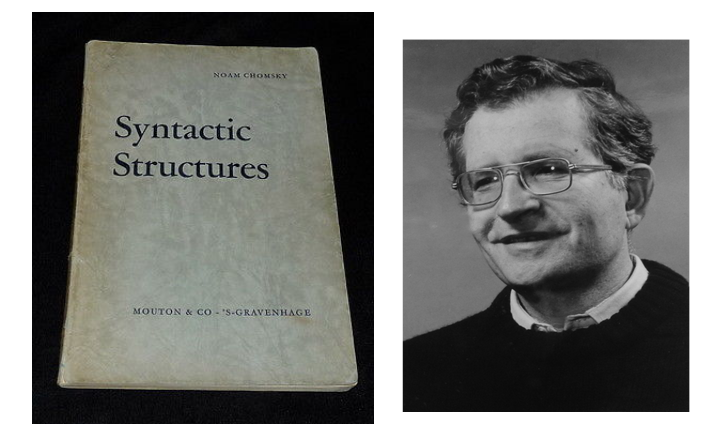
\includegraphics[scale = 0.4]{pics/chomsky.png}
        \end{figure}      
\end{frame}

\begin{frame}{The Bias-Variance Trade-Off}
    \scriptsize
    \begin{itemize}
        \item Trigram maximum-likelihood estimate:
        \[
        q_{\text{ML}}(w_i | w_{i-2}, w_{i-1}) = \frac{{\text{Count}(w_{i-2}, w_{i-1}, w_i)}}{{\text{Count}(w_{i-2}, w_{i-1})}}
        \]
        \item Bigram maximum-likelihood estimate:
        \[
        q_{\text{ML}}(w_i | w_{i-1}) = \frac{{\text{Count}(w_{i-1}, w_i)}}{{\text{Count}(w_{i-1})}}
        \]
        \item Unigram maximum-likelihood estimate:
        \[
        q_{\text{ML}}(w_i) = \frac{{\text{Count}(w_i)}}{{\text{Count()}}}
        \]
    \end{itemize}
\end{frame}

\begin{frame}{Linear Interpolation}
    \scriptsize
    \begin{itemize}
     \item Take our estimate $q(w_i | w_{i-2}, w_{i-1})$ to be
    \[
    q(w_i | w_{i-2}, w_{i-1}) = \lambda_1 \cdot q_{\text{ML}}(w_i | w_{i-2}, w_{i-1}) + \lambda_2 \cdot q_{\text{ML}}(w_i | w_{i-1}) + \lambda_3 \cdot q_{\text{ML}}(w_i)
    \]
    where $\lambda_1 + \lambda_2 + \lambda_3 = 1$, and $\lambda_i \geq 0$ for all $i$.
    
    \item Our estimate correctly defines a distribution (define $V' = V \cup \{\text{STOP}\}$):
    \[
    \begin{aligned}
        & \sum_{w \in V'} q(w | u, v) \\
        = & \sum_{w \in V'} [\lambda_1 \cdot q_{\text{ML}}(w | u, v) + \lambda_2 \cdot q_{\text{ML}}(w | v) + \lambda_3 \cdot q_{\text{ML}}(w)] \\
        = & \lambda_1 \sum_{w} q_{\text{ML}}(w | u, v) + \lambda_2 \sum_{w} q_{\text{ML}}(w | v) + \lambda_3 \sum_{w} q_{\text{ML}}(w) \\
        = & \lambda_1 + \lambda_2 + \lambda_3 = 1
    \end{aligned}
    \]
    \item We can also show that $q(w | u, v) \geq 0$ for all $w \in V'$.
    \end{itemize}

    
    
\end{frame}

\begin{frame}{Estimating $\lambda$ Values}
\scriptsize
\begin{itemize}
  \item Hold out part of the training set as \textit{validation} data.
  \item Define $c'(w_1, w_2, w_3)$ to be the number of times the trigram $(w_1, w_2, w_3)$ is seen in the validation set.
  \item Choose $\lambda_1$, $\lambda_2$, $\lambda_3$ to maximize:
  \[
  L(\lambda_1, \lambda_2, \lambda_3) = \sum_{w_1,w_2,w_3} c'(w_1, w_2, w_3) \log q(w_3 | w_1, w_2)
  \]
  such that $\lambda_1 + \lambda_2 + \lambda_3 = 1$, and $\lambda_i \geq 0$ for all $i$, and where
  \[
  q(w_i | w_{i-2}, w_{i-1}) = \lambda_1 \cdot q_{\text{ML}}(w_i | w_{i-2}, w_{i-1}) + \lambda_2 \cdot q_{\text{ML}}(w_i | w_{i-1}) + \lambda_3 \cdot q_{\text{ML}}(w_i)
  \]
\end{itemize}
\end{frame}



\begin{frame}{Discounting Methods}
\begin{scriptsize}
\begin{itemize}
\item Consider the following counts and maximum-likelihood estimates:
\end{itemize}

\begin{table}[h]
    \centering
    \begin{tabular}{lll}
        \textbf{Sentence} & \textbf{Count} & \textbf{$q_{\text{ML}}(w_i | w_{i-1})$} \\
        \hline
        the & 48 & \\
        the, dog & 15 & $15/48$ \\
        the, woman & 11 & $11/48$ \\
        the, man & 10 & $10/48$ \\
        the, park & 5 & $5/48$ \\
        the, job & 2 & $2/48$ \\
        the, telescope & 1 & $1/48$ \\
        the, manual & 1 & $1/48$ \\
        the, afternoon & 1 & $1/48$ \\
        the, country & 1 & $1/48$ \\
        the, street & 1 & $1/48$ \\
    \end{tabular}
\end{table}

\begin{itemize}
    \item The maximum-likelihood estimates are high, particularly for low count items.
\end{itemize}
\end{scriptsize}
\end{frame}



\begin{frame}{Discounting Methods}
\begin{scriptsize}
\begin{itemize}
\item Define ``discounted'' counts as follows:
\begin{displaymath}
\text{Count}^*(x) =\text{Count}(x)-0.5
\end{displaymath}

\end{itemize}

\begin{table}[h]
    \centering
    \begin{tabular}{llll}
        \textbf{Sentence} & \textbf{Count} & \textbf{Count}*$\mathbf{(x)}$ & $\mathbf{q_{\text{ML}}(w_i | w_{i-1})}$ \\
        \hline
        the & 48 & & \\
        the, dog & 15 & 14.5 & $14.5/48$ \\
        the, woman & 11 & 10.5 & $10.5/48$ \\
        the, man & 10 & 9.5 & $9.5/48$ \\
        the, park & 5 & 4.5 & $4.5/48$ \\
        the, job & 2 & 1.5 & $1.5/48$ \\
        the, telescope & 1 & 0.5 & $0.5/48$ \\
        the, manual & 1 & 0.5 & $0.5/48$ \\
        the, afternoon & 1 & 0.5 & $0.5/48$ \\
        the, country & 1 & 0.5 & $0.5/48$ \\
        the, street & 1 & 0.5 & $0.5/48$ \\
    \end{tabular}
\end{table}

\begin{itemize}
    \item The new estimates are based on the discounted counts.
\end{itemize}
\end{scriptsize}
\end{frame}



\begin{frame}{Discounting Methods (Continued)}
    \begin{itemize}
        \item We now have some "missing probability mass":
        \[
        \alpha(w_{i-1}) = 1 - \sum_{w} \frac{{\text{{Count}}^*(w_{i-1}, w)}}{{\text{{Count}}(w_{i-1})}}
        \]
        \item For example, in our case:
        \[
        \alpha(\text{{the}}) = \frac{{10 \times 0.5}}{{48}} = \frac{{5}}{{48}}
        \]
    \end{itemize}
\end{frame}

\begin{frame}{Katz Back-Off Models (Bigrams)}
    \begin{itemize}
        \item For a bigram model, define two sets:
        \[
        A(w_{i-1}) = \{w : \text{Count}(w_{i-1}, w) > 0\}
        \]
        \[
        B(w_{i-1}) = \{w : \text{Count}(w_{i-1}, w) = 0\}
        \]
        \item A bigram model:
        \[
        q_{\text{BO}}(w_i | w_{i-1}) =
        \begin{cases}
            \frac{\text{Count}^*(w_{i-1}, w_i)}{\text{Count}(w_{i-1})} & \text{if } w_i \in A(w_{i-1}) \\
            \frac{\alpha(w_{i-1}) q_{\text{ML}}(w_i)}{\sum_{w \in B(w_{i-1})} q_{\text{ML}}(w)} & \text{if } w_i \in B(w_{i-1})
        \end{cases}
        \]
        \item Where:
        \[
        \alpha(w_{i-1}) = 1 - \sum_{w \in A(w_{i-1})} \frac{\text{Count}^*(w_{i-1}, w)}{\text{Count}(w_{i-1})}
        \]
    \end{itemize}
\end{frame}

\begin{frame}{Katz Back-Off Models (Trigrams)}
\begin{scriptsize}
    \begin{itemize}
        \item For a trigram model, first define two sets:
        \[
        A(w_{i-2}, w_{i-1}) = \{w : \text{Count}(w_{i-2}, w_{i-1}, w) > 0\}
        \]
        \[
        B(w_{i-2}, w_{i-1}) = \{w : \text{Count}(w_{i-2}, w_{i-1}, w) = 0\}
        \]
        \item A trigram model is defined in terms of the bigram model:
        \[
        q_{\text{BO}}(w_i | w_{i-2}, w_{i-1}) =
        \begin{cases}
            \frac{\text{Count}^*(w_{i-2}, w_{i-1}, w_i)}{\text{Count}(w_{i-2}, w_{i-1})} & \text{if } w_i \in A(w_{i-2}, w_{i-1}) \\
            \frac{\alpha(w_{i-2}, w_{i-1}) q_{\text{BO}}(w_i|w_{i-1})}{\sum_{w \in B(w_{i-2}, w_{i-1})} q_{\text{BO}}(w|w_{i-1})} & \text{if } w_i \in B(w_{i-2}, w_{i-1})
        \end{cases}
        \]
        \item Where:
        \[
        \alpha(w_{i-2}, w_{i-1}) = 1 - \sum_{w \in A(w_{i-2}, w_{i-1})} \frac{\text{Count}^*(w_{i-2}, w_{i-1}, w)}{\text{Count}(w_{i-2}, w_{i-1})}
        \]
    \end{itemize}
    
    \end{scriptsize}
\end{frame}

\begin{frame}{Summary}
    \scriptsize
    \begin{itemize}
        \item Deriving probabilities in probabilistic language models involves three steps:
        \begin{enumerate}\scriptsize{
            \item Expand $p(w_1, w_2, \ldots, w_n)$ using the Chain rule.
            \item Apply Markov Independence Assumptions \\
            $p(w_i | w_1, w_2, \ldots, w_{i-2}, w_{i-1}) = p(w_i | w_{i-2}, w_{i-1})$.
            \item Smooth the estimates using low order counts.}
        \end{enumerate}
        \item Other methods for improving language models include:
        \begin{itemize}\scriptsize{
            \item Introducing latent variables to represent topics, known as topic models. \cite{blei2003latent}
            \item Replacing $p(w_i | w_1, w_2, \ldots, w_{i-2}, w_{i-1})$ with a predictive neural network and an ``embedding layer'' to better represent larger contexts and leverage similarities between words in the context. \cite{bengio2000neural}}
        \end{itemize}
        \item Modern language models utilize deep neural networks in their backbone and have a vast parameter space.
    \end{itemize}
\end{frame}


\begin{frame}
\frametitle{Questions?}
%\vspace{1.5cm}
\begin{center}\LARGE Thanks for your Attention!\\ \end{center}



\end{frame}




\begin{frame}[allowframebreaks]\scriptsize
\frametitle{References}
\bibliography{bio}
\bibliographystyle{apalike}
%\bibliographystyle{flexbib}
\end{frame}  


%%%%%%%%%%%%%%%%%%%%%%%%%%%

\end{document}
